%\documentclass{article}
%\usepackage{beamerarticle}
\documentclass[serif,ignorenonframetext]{beamer}

% Macros for MATH 110 course dates

\newcommand{\commonTheme}{metropolis}
\newcommand{\commonColorTheme}{metropolis}

\newcommand{\commonAuthor}{Edward Doolittle}
\newcommand{\commonInstitute}{Department of Indigenous Knowledge and
  Science \\ First Nations University of Canada}
\newcommand{\commonCourse}{MATH 110 Calculus I}
\newcommand{\commonTerm}{202510}
\newcommand{\commonDate}{January 6, 2025}

% Review Material

% Lab 0
\newcommand{\commonEventNegativeOne}{LabNegativeOne}
\newcommand{\commonDateLabNegativeOne}{Monday, January 6, 2025}
\newcommand{\commonTitleLabNegativeOne}{MATH 110 Lab 0}
\newcommand{\commonSubtitleLabNegativeOne}{No Lab; Course Opens}

% Section 001
\newcommand{\commonEventZeroZeroOne}{ZeroZeroOne}
\newcommand{\commonDateZeroZeroOne}{Tuesday, January 7, 2025}
\newcommand{\commonTitleZeroZeroOne}{MATH 110 Review 0.1}
\newcommand{\commonSubtitleZeroZeroOne}{Review of Algebra}
\newcommand{\commonPSTitleZeroZeroOne}{MATH 110 Review Problem Set 0.1}

% Section 00A
\newcommand{\commonEventZeroZeroA}{ZeroZeroA}
\newcommand{\commonDateZeroZeroA}{Tuesday, January 7, 2025}
\newcommand{\commonTitleZeroZeroA}{MATH 110 Review 0.A}
\newcommand{\commonSubtitleZeroZeroA}{Review of Inequalities and
  Absolute Values}
\newcommand{\commonPSTitleZeroZeroA}{MATH 110 Review Problem Set 0.A}

% Section 00B
\newcommand{\commonEventZeroZeroB}{ZeroZeroB}
\newcommand{\commonDateZeroZeroB}{Tuesday, January 7, 2025}
\newcommand{\commonTitleZeroZeroB}{MATH 110 Review 0.B}
\newcommand{\commonSubtitleZeroZeroB}{Review of Coordinate Geometry
  and Lines}
\newcommand{\commonPSTitleZeroZeroB}{MATH 110 Review Problem Set 0.B}

% Section 00C
\newcommand{\commonEventZeroZeroC}{ZeroZeroC}
\newcommand{\commonDateZeroZeroC}{Thursday, January 9, 2025}
\newcommand{\commonTitleZeroZeroC}{MATH 110 Review 0.C}
\newcommand{\commonSubtitleZeroZeroC}{Review of Graphs of Second
  Degree Equations}
\newcommand{\commonPSTitleZeroZeroC}{MATH 110 Review Problem Set 0.C}

% Section 00D
\newcommand{\commonEventZeroZeroD}{ZeroZeroD}
\newcommand{\commonDateZeroZeroD}{Thursday, January 9, 2025}
\newcommand{\commonTitleZeroZeroD}{MATH 110 Review 0.D}
\newcommand{\commonSubtitleZeroZeroD}{Review of Trigonometry}
\newcommand{\commonPSTitleZeroZeroD}{MATH 110 Review Problem Set 0.D}

% Section 011
\newcommand{\commonEventZeroOneOne}{ZeroOneOne}
\newcommand{\commonDateZeroOneOne}{Thursday, January 9, 2025}
\newcommand{\commonTitleZeroOneOne}{MATH 110 Review 1.1}
\newcommand{\commonSubtitleZeroOneOne}{Review of Functions}
\newcommand{\commonPSTitleZeroOneOne}{MATH 110 Review Problem Set 1.1}


% Main Course

% Lab 1
\newcommand{\commonEventZero}{LabZero}
\newcommand{\commonDateLabZero}{Monday, January 13, 2025}
\newcommand{\commonTitleLabZero}{MATH 110 Lab 1}
\newcommand{\commonSubtitleLabZero}{Quiz 0: STACK, Onboarding}

% Section 1.4
\newcommand{\commonEventOne}{ZeroOneFour}
\newcommand{\commonDateZeroOneFour}{Tuesday, January 14, 2025}
\newcommand{\commonTitleZeroOneFour}{MATH 110 Lecture 1.4}
\newcommand{\commonSubtitleZeroOneFour}{The Tangent and Velocity Problems}
\newcommand{\commonPSTitleZeroOneFour}{MATH 110 Problem Set 1.4}

% Section 1.5
\newcommand{\commonEventTwo}{ZeroOneFive}
\newcommand{\commonDateZeroOneFive}{Thursday, January 16, 2025}
\newcommand{\commonTitleZeroOneFive}{MATH 110 Lecture 1.5}
\newcommand{\commonSubtitleZeroOneFive}{The Limit of a Function}
\newcommand{\commonPSTitleZeroOneFive}{MATH 110 Problem Set 1.5}

% Lab 2
\newcommand{\commonEventThree}{LabOne}
\newcommand{\commonDateLabOne}{Monday, January 20, 2025}
\newcommand{\commonTitleLabOne}{MATH 110 Lab 2}
\newcommand{\commonSubtitleLabOne}{Quiz 1: Review}

% Section 1.6
\newcommand{\commonEventFour}{ZeroOneSix}
\newcommand{\commonDateZeroOneSix}{Tuesday, January 21, 2025}
\newcommand{\commonTitleZeroOneSix}{MATH 110 Lecture 1.6}
\newcommand{\commonSubtitleZeroOneSix}{Calculating Limits Using the Limit Laws}
\newcommand{\commonPSTitleZeroOneSix}{MATH 110 Problem Set 1.6}

% Section 1.7
\newcommand{\commonEventFive}{ZeroOneSeven}
\newcommand{\commonDateZeroOneSeven}{(Not covered)}
\newcommand{\commonTitleZeroOneSeven}{MATH 110 Lecture 1.7}
\newcommand{\commonSubtitleZeroOneSeven}{The Precise Definition of a Limit}
\newcommand{\commonPSTitleZeroOneSeven}{MATH 110 Problem Set 1.7}

% Section 1.8
\newcommand{\commonEventSix}{ZeroOneEight}
\newcommand{\commonDateZeroOneEight}{Thursday, January 23, 2025}
\newcommand{\commonTitleZeroOneEight}{MATH 110 Lecture 1.8}
\newcommand{\commonSubtitleZeroOneEight}{Continuity}
\newcommand{\commonPSTitleZeroOneEight}{MATH 110 Problem Set 1.8}

% Lab 3
\newcommand{\commonEventSeven}{LabTwo}
\newcommand{\commonDateLabTwo}{Monday, January 27, 2025}
\newcommand{\commonTitleLabTwo}{MATH 110 Lab 3}
\newcommand{\commonSubtitleLabTwo}{Quiz 2: Sections 1.4, 1.5}

% Section 2.1
\newcommand{\commonEventEight}{ZeroTwoOne}
\newcommand{\commonDateZeroTwoOne}{Tuesday, January 28, 2025}
\newcommand{\commonTitleZeroTwoOne}{MATH 110 Lecture 2.1}
\newcommand{\commonSubtitleZeroTwoOne}{Derivatives and Rates of Change}
\newcommand{\commonPSTitleZeroTwoOne}{MATH 110 Problem Set 2.1}

% Section 2.2
\newcommand{\commonEventNine}{ZeroTwoTwo}
\newcommand{\commonDateZeroTwoTwo}{Thursday, January 30, 2025}
\newcommand{\commonTitleZeroTwoTwo}{MATH 110 Lecture 2.2}
\newcommand{\commonSubtitleZeroTwoTwo}{The Derivative as a Function}
\newcommand{\commonPSTitleZeroTwoTwo}{MATH 110 Problem Set 2.2}

% Lab 4
\newcommand{\commonEventTen}{LabThree}
\newcommand{\commonDateMTOne}{Monday, February 3, 2025} 
\newcommand{\commonDateLabThree}{Monday, February 3, 2025}
\newcommand{\commonTitleLabThree}{MATH 110 Lab 4}
\newcommand{\commonSubtitleLabThree}{Midterm: Review, Chapter 1}

% Section 2.3
\newcommand{\commonEventEleven}{ZeroTwoThree}
\newcommand{\commonDateZeroTwoThree}{Tuesday, February 4, 2025}
\newcommand{\commonTitleZeroTwoThree}{MATH 110 Lecture 2.3}
\newcommand{\commonSubtitleZeroTwoThree}{Differentiation Formulas}
\newcommand{\commonPSTitleZeroTwoThree}{MATH 110 Problem Set 2.3}

% Section 2.4
\newcommand{\commonEventTwelve}{ZeroTwoFour}
\newcommand{\commonDateZeroTwoFour}{Thursday, February 6, 2025}
\newcommand{\commonTitleZeroTwoFour}{MATH 110 Lecture 2.4}
\newcommand{\commonSubtitleZeroTwoFour}{Derivatives of Trigonometric Functions}
\newcommand{\commonPSTitleZeroTwoFour}{MATH 110 Problem Set 2.4}

% Lab 5
\newcommand{\commonEventThirteen}{LabFour}
\newcommand{\commonDateLabFour}{Monday, February 10, 2025}
\newcommand{\commonTitleLabFour}{MATH 110 Lab 5}
\newcommand{\commonSubtitleLabFour}{Quiz 3: Sections 2.1, 2.2}

% Section 2.5
\newcommand{\commonEventFourteen}{ZeroTwoFive}
\newcommand{\commonDateZeroTwoFive}{Tuesday, February 11, 2025}
\newcommand{\commonTitleZeroTwoFive}{MATH 110 Lecture 2.5}
\newcommand{\commonSubtitleZeroTwoFive}{The Chain Rule}
\newcommand{\commonPSTitleZeroTwoFive}{MATH 110 Problem Set 2.5}

% Section 2.6
\newcommand{\commonEventFifteen}{ZeroTwoSix}
\newcommand{\commonDateZeroTwoSix}{Thursday, February 13, 2025}
\newcommand{\commonTitleZeroTwoSix}{MATH 110 Lecture 2.6}
\newcommand{\commonSubtitleZeroTwoSix}{Implicit Differentiation}
\newcommand{\commonPSTitleZeroTwoSix}{MATH 110 Problem Set 2.6}

% Lab 6
\newcommand{\commonEventSixteen}{LabFive}
\newcommand{\commonDateLabFive}{Monday, February 24, 2025}
\newcommand{\commonTitleLabFive}{MATH 110 Lab 6}
\newcommand{\commonSubtitleLabFive}{Quiz 4: Sections 2.3, 2.4}

% Section 2.7
\newcommand{\commonEventSeventeen}{ZeroTwoSeven}
\newcommand{\commonDateZeroTwoSeven}{Tuesday, February 25, 2025}
\newcommand{\commonTitleZeroTwoSeven}{MATH 110 Lecture 2.7}
\newcommand{\commonSubtitleZeroTwoSeven}{Rates of Change in the
  Natural and Social Sciences}
\newcommand{\commonPSTitleZeroTwoSeven}{MATH 110 Problem Set 2.7}

% Section 2.8
\newcommand{\commonEventEighteen}{ZeroTwoEight}
\newcommand{\commonDateZeroTwoEight}{Thursday, February 27, 2025}
\newcommand{\commonTitleZeroTwoEight}{MATH 110 Lecture 2.8}
\newcommand{\commonSubtitleZeroTwoEight}{Related Rates}
\newcommand{\commonPSTitleZeroTwoEight}{MATH 110 Problem Set 2.8}

% Lab 7
\newcommand{\commonEventNineteen}{LabSix}
\newcommand{\commonDateLabSix}{Monday, March 3, 2025}
\newcommand{\commonTitleLabSix}{MATH 110 Lab 7}
\newcommand{\commonSubtitleLabSix}{Quiz 5: Sections 2.5, 2.6}

% Section 3.1
\newcommand{\commonEventTwenty}{ZeroThreeOne}
\newcommand{\commonDateZeroThreeOne}{Tuesday, March 4, 2025}
\newcommand{\commonTitleZeroThreeOne}{MATH 110 Lecture 3.1}
\newcommand{\commonSubtitleZeroThreeOne}{Maximum and Minimum Values}
\newcommand{\commonPSTitleZeroThreeOne}{MATH 11 Problem Set 3.1}

% Section 3.2
\newcommand{\commonEventTwentyOne}{ZeroThreeTwo}
\newcommand{\commonDateZeroThreeTwo}{Thursday, March 6, 2025}
\newcommand{\commonTitleZeroThreeTwo}{MATH 110 Lecture 3.2}
\newcommand{\commonSubtitleZeroThreeTwo}{The Mean Value Theorem}
\newcommand{\commonPSTitleZeroThreeTwo}{MATH 110 Problem Set 3.2}

% Lab 8
\newcommand{\commonEventTwentyTwo}{LabSeven}
\newcommand{\commonDateMTTwo}{Monday, March 10, 2025}
\newcommand{\commonDateLabSeven}{Monday, March 10, 2025}
\newcommand{\commonTitleLabSeven}{MATH 110 Lab 8}
\newcommand{\commonSubtitleLabSeven}{Midterm: Chapter 2}

% Section 3.3
\newcommand{\commonEventTwentyThree}{ZeroThreeThree}
\newcommand{\commonDateZeroThreeThree}{Tuesday, March 11, 2025}
\newcommand{\commonTitleZeroThreeThree}{MATH 110 Lecture 3.3}
\newcommand{\commonSubtitleZeroThreeThree}{How Derivatives Affect the
  Shape of a Graph}
\newcommand{\commonPSTitleZeroThreeThree}{MATH 110 Problem Set 3.3}

% Section 3.4
\newcommand{\commonEventTwentyFour}{ZeroThreeFour}
\newcommand{\commonDateZeroThreeFour}{Thursday, March 13, 2025}
\newcommand{\commonTitleZeroThreeFour}{MATH 110 Lecture 3.4}
\newcommand{\commonSubtitleZeroThreeFour}{Limits at Infinity;
  Horizontal Asymptotes}
\newcommand{\commonPSTitleZeroThreeFour}{MATH 110 Problem Set 3.4}

% Lab 9
\newcommand{\commonEventTwentyFive}{LabEight}
\newcommand{\commonDateLabEight}{Monday, March 17, 2025}
\newcommand{\commonTitleLabEight}{MATH 110 Lab 9}
\newcommand{\commonSubtitleLabEight}{Quiz 6: Sections 3.1, 3.2}

% Section 3.5
\newcommand{\commonEventTwentySix}{ZeroThreeFive}
\newcommand{\commonDateZeroThreeFive}{Tuesday, March 18, 2025}
\newcommand{\commonTitleZeroThreeFive}{MATH 110 Lecture 3.5}
\newcommand{\commonSubtitleZeroThreeFive}{Summary of Curve Sketching}
\newcommand{\commonPSTitleZeroThreeFive}{MATH 110 Problem Set 3.5}

% Section 3.7
\newcommand{\commonEventTwentySeven}{ZeroThreeSeven}
\newcommand{\commonDateZeroThreeSeven}{Thursday, March 20, 2025}
\newcommand{\commonTitleZeroThreeSeven}{MATH 110 Lecture 3.7}
\newcommand{\commonSubtitleZeroThreeSeven}{Optimization Problems}
\newcommand{\commonPSTitleZeroThreeSeven}{MATH 110 Problem Set 3.7}

% Lab 10
\newcommand{\commonEventTwentyEight}{LabNine}
\newcommand{\commonDateLabNine}{Monday, March 24, 2025}
\newcommand{\commonTitleLabNine}{MATH 110 Lab 10}
\newcommand{\commonSubtitleLabNine}{Quiz 7: Sections 3.3, 3.4}

% Section 4.1
\newcommand{\commonEventTwentyNine}{ZeroFourOne}
\newcommand{\commonDateZeroFourOne}{Tuesday, March 25, 2025}
\newcommand{\commonTitleZeroFourOne}{MATH 110 Lecture 4.1}
\newcommand{\commonSubtitleZeroFourOne}{Areas and Distances}
\newcommand{\commonPSTitleZeroFourOne}{MATH 110 Problem Set 4.1}

% Section 4.2
\newcommand{\commonEventThirty}{ZeroFourTwo}
\newcommand{\commonDateZeroFourTwo}{Thursday, March 27, 2025}
\newcommand{\commonTitleZeroFourTwo}{MATH 110 Lecture 4.2}
\newcommand{\commonSubtitleZeroFourTwo}{The Definite Integral}
\newcommand{\commonPSTitleZeroFourTwo}{MATH 110 Problem Set 4.2}

% Lab 11
\newcommand{\commonEventThirtyOne}{LabTen}
\newcommand{\commonDateLabTen}{Monday, March 31, 2025}
\newcommand{\commonTitleLabTen}{MATH 110 Lab 11}
\newcommand{\commonSubtitleLabTen}{Quiz 8: Sections 3.5, 3.7}

% Section 4.3
\newcommand{\commonEventThirtyTwo}{ZeroFourThree}
\newcommand{\commonDateZeroFourThree}{Tuesday, April 1, 2025}
\newcommand{\commonTitleZeroFourThree}{MATH 110 Lecture 4.3}
\newcommand{\commonSubtitleZeroFourThree}{The Fundamental Theorem of Calculus}
\newcommand{\commonPSTitleZeroFourThree}{MATH 110 Problem Set 4.3}

% Section 4.4
\newcommand{\commonEventThirtyThree}{ZeroFourFour}
\newcommand{\commonDateZeroFourFour}{Thursday, April 3, 2025}
\newcommand{\commonTitleZeroFourFour}{MATH 110 Lecture 4.4}
\newcommand{\commonSubtitleZeroFourFour}{Indefinite Integrals and the
  Net Change Theorem}
\newcommand{\commonPSTitleZeroFourFour}{MATH 110 Problem Set 4.4}

% Lab 12
\newcommand{\commonEventThirtyFour}{LabEleven}
\newcommand{\commonDateLabEleven}{Monday, April 7, 2025}
\newcommand{\commonTitleLabEleven}{MATH 110 Lab 12}
\newcommand{\commonSubtitleLabEleven}{Quiz 9: Sections 4.1, 4.2}

% Section 4.5
\newcommand{\commonEventThirtyFive}{ZeroFourFive}
\newcommand{\commonDateZeroFourFive}{Tuesday, April 8, 2025}
\newcommand{\commonTitleZeroFourFive}{MATH 110 Lecture 4.5}
\newcommand{\commonSubtitleZeroFourFive}{The Substitution Rule}
\newcommand{\commonPSTitleZeroFourFive}{MATH 110 Problem Set 4.5}

% Section 5.1
\newcommand{\commonEventThirtySix}{ZeroFiveOne}
\newcommand{\commonDateZeroFiveOne}{Thursday, April 10, 2025}
\newcommand{\commonTitleZeroFiveOne}{MATH 110 Lecture 5.1}
\newcommand{\commonSubtitleZeroFiveOne}{Areas Between Curves}
\newcommand{\commonPSTitleZeroFiveOne}{MATH 110 Problem Set 5.1}

% Lab 13
\newcommand{\commonEventThirtySeven}{LabTwelve}
\newcommand{\commonDateLabTwelve}{Monday, April 14, 2025}
\newcommand{\commonTitleLabTwelve}{MATH 110 Review Lab}
\newcommand{\commonSubtitleLabTwelve}{Bonus Quiz 10: Sections 4.3, 4.4}

% Final Class
\newcommand{\commonEventThirtyEight}{FinalClass}
\newcommand{\commonDateFinalClass}{Tuesday, April 15, 2025}
\newcommand{\commonTitleFinalClass}{MATH 110 Review Class}
\newcommand{\commonSubtitleFinalClass}{Answer Questions, Review for Exam}

% Final Exam
\newcommand{\commonEventThirtyNine}{Final}
\newcommand{\commonDateFinal}{Thursday, April 22, 2025}
\newcommand{\commonTitleFinal}{MATH 110 Final Exam}
\newcommand{\commonSubtitleFinal}{Comprehensive Exam: All Sections}

% Orphaned -- no longer part of the course

% Section 2.9
\newcommand{\commonDateZeroTwoNine}{Not part of the course}
\newcommand{\commonTitleZeroTwoNine}{MATH 110 Lecture 2.9}
\newcommand{\commonSubtitleZeroTwoNine}{Linear Approximations and Differentials}
\newcommand{\commonPSTitleZeroTwoNine}{MATH 110 Problem Set 2.9}


% % Introduction
% \newcommand{\commonEventOneDate}{Wednesday, September 8, 2010}
% \newcommand{\commonEventOneDesc}{Introduction to the Course}
% \newcommand{\commonDateZeroZeroZero}{September 8, 2010}
% \newcommand{\commonTitleZeroZeroZero}{MATH 104 Introduction}
% \newcommand{\commonSubtitleZeroZeroZero}{Outline of the Course}

% % Lecture 1
% \newcommand{\commonEventTwoDate}{Friday, September 10, 2010}
% \newcommand{\commonEventTwoDesc}{Lecture 1: Algebra}
% \newcommand{\commonDateZeroZeroOne}{September 10, 2010}
% \newcommand{\commonTitleZeroZeroOne}{MATH 104 Lecture 1}
% \newcommand{\commonSubtitleZeroZeroOne}{Review of Algebra}
% % associated evaluation ... factor this out?
% \newcommand{\commonPSTitleZeroZeroOne}{MATH 104 Problem Set 1}
% \newcommand{\commonEvalZeroZeroOne}{Quiz 1}
% \newcommand{\commonEvalDateZeroZeroOne}{Wednesday, September 15, 2010}

% % Lecture 2
% \newcommand{\commonEventThreeDate}{Monday, September 13, 2010}
% \newcommand{\commonEventThreeDesc}{Lecture 2: Appendix A}
% \newcommand{\commonDateZeroZeroA}{September 13, 2010}
% \newcommand{\commonTitleZeroZeroA}{MATH 104 Lecture 2}
% \newcommand{\commonSubtitleZeroZeroA}{Appendix A: Numbers, Inequalities, 
%   and Absolute Values}
% % associated evaluation ... factor this out?
% \newcommand{\commonPSTitleZeroZeroA}{MATH 104 Problem Set 2}
% \newcommand{\commonEvalZeroZeroA}{Quiz 2}
% \newcommand{\commonEvalDateZeroZeroA}{Wednesday, September 22, 2010}

% % Review 1
% \newcommand{\commonEventFourDate}{Wednesday, September 15, 2010}
% \newcommand{\commonEventFourDesc}{Review 1: Review Algebra; Quiz 1; Review Appendix A}
% \newcommand{\commonDateRZeroOne}{September 15, 2010}
% \newcommand{\commonTitleRZeroOne}{MATH 104 Review 1}
% \newcommand{\commonSubtitleRZeroOne}{Review of Algebra, Appendix A}

% % Lecture 3
% \newcommand{\commonEventFiveDate}{Friday, September 17, 2010}
% \newcommand{\commonEventFiveDesc}{Lecture 3: Appendix B}
% \newcommand{\commonDateZeroZeroB}{September 17, 2010}
% \newcommand{\commonTitleZeroZeroB}{MATH 104 Lecture 3}
% \newcommand{\commonSubtitleZeroZeroB}{Appendix B: Coordinate Geometry and Lines}
% % associated evaluation ... factor this out?
% \newcommand{\commonPSTitleZeroZeroB}{MATH 104 Problem Set 3}
% \newcommand{\commonEvalZeroZeroB}{Quiz 2}
% \newcommand{\commonEvalDateZeroZeroB}{Wednesday, September 22, 2010}

% % Lecture 4
% \newcommand{\commonEventSixDate}{Monday, Sepbember 20, 2010}
% \newcommand{\commonEventSixDesc}{Lecture 4: Appendix C}
% \newcommand{\commonDateZeroZeroC}{September 20, 2010}
% \newcommand{\commonTitleZeroZeroC}{MATH 104 Lecture 4}
% \newcommand{\commonSubtitleZeroZeroC}{Appendix C: Graphs of Second-Degree Equations}
% % associated evaluation ... factor this out?
% \newcommand{\commonPSTitleZeroZeroC}{MATH 104 Problem Set 4}
% \newcommand{\commonEvalZeroZeroC}{Midterm 0}
% \newcommand{\commonEvalDateZeroZeroC}{Wednesday, September 29, 2010}

% % Review 2
% \newcommand{\commonEventSevenDate}{Wednesday, September 22, 2010}
% \newcommand{\commonEventSevenDesc}{Review 2: Review Appendix B; Quiz 2; Review Appendix C}
% \newcommand{\commonDateRZeroTwo}{September 22, 2010}
% \newcommand{\commonTitleRZeroTwo}{MATH 104 Review 2}
% \newcommand{\commonSubtitleRZeroTwo}{Review of Appendices B and C}

% % Lecture 5
% \newcommand{\commonEventEightDate}{Friday, September 24, 2010}
% \newcommand{\commonEventEightDesc}{Lecture 5: Appendix D}
% \newcommand{\commonDateZeroZeroD}{September 24, 2010}
% \newcommand{\commonTitleZeroZeroD}{MATH 104 Lecture 5}
% \newcommand{\commonSubtitleZeroZeroD}{Appendix D: Trigonometry}
% % associated evaluation ... factor this out?
% \newcommand{\commonPSTitleZeroZeroD}{MATH 104 Problem Set 5}
% \newcommand{\commonEvalZeroZeroD}{Midterm 0}
% \newcommand{\commonEvalDateZeroZeroD}{Wednesday, September 29, 2010}

% % Lecture 6
% \newcommand{\commonEventNineDate}{Monday, September 27, 2010}
% \newcommand{\commonEventNineDesc}{Lecture 6: Section 1.1}
% \newcommand{\commonDateZeroOneOne}{September 27, 2010}
% \newcommand{\commonTitleZeroOneOne}{MATH 104 Lecture 6}
% \newcommand{\commonSubtitleZeroOneOne}{Section 1.1: Four Ways to Represent a Function}
% % associated evaluation ... factor this out?
% \newcommand{\commonPSTitleZeroOneOne}{MATH 104 Problem Set 6}
% \newcommand{\commonEvalZeroOneOne}{Quiz 3}
% \newcommand{\commonEvalDateZeroOneOne}{Wednesday, October 6, 2010}

% % Review 3
% \newcommand{\commonEventTenDate}{Wednesday, September 29, 2010}
% \newcommand{\commonEventTenDesc}{Review 3: Review Appendix D; 
%   Self-Assessment Midterm 0}
% \newcommand{\commonDateRZeroThree}{September 29, 2010}
% \newcommand{\commonTitleRZeroThree}{MATH 104 Review 3}
% \newcommand{\commonSubtitleRZeroThree}{Review of Appendix D}

% % Lecture 7
% \newcommand{\commonEventElevenDate}{Friday, October 1, 2010}
% \newcommand{\commonEventElevenDesc}{Lecture 7: Section 1.2}
% \newcommand{\commonDateZeroOneTwo}{October 1, 2010}
% \newcommand{\commonTitleZeroOneTwo}{MATH 104 Lecture 7}
% \newcommand{\commonSubtitleZeroOneTwo}{Section 1.2: Mathematical Models: A Catalog of Essential Functions}
% % associated evaluation ... factor this out?
% \newcommand{\commonPSTitleZeroOneTwo}{MATH 104 Problem Set 7}
% \newcommand{\commonEvalZeroOneTwo}{Quiz 3}
% \newcommand{\commonEvalDateZeroOneTwo}{Wednesday, October 6, 2010}

% % Lecture 8
% \newcommand{\commonEventTwelveDate}{Monday, October 4, 2010}
% \newcommand{\commonEventTwelveDesc}{Lecture 8: Section 1.3}
% \newcommand{\commonDateZeroOneThree}{October 4, 2010}
% \newcommand{\commonTitleZeroOneThree}{MATH 104 Lecture 8}
% \newcommand{\commonSubtitleZeroOneThree}{Section 1.3: New Functions from Old Functions}
% % associated evaluation ... factor this out?
% \newcommand{\commonPSTitleZeroOneThree}{MATH 104 Problem Set 8}
% \newcommand{\commonEvalZeroOneThree}{Quiz 4}
% \newcommand{\commonEvalDateZeroOneThree}{Wednesday, October 13, 2010}

% % Review 4
% \newcommand{\commonEventThirteenDate}{Wednesday, October 6, 2010}
% \newcommand{\commonEventThirteenDesc}{Review 4: Review 1.1, 1.2; Quiz 3}
% \newcommand{\commonDateROneOne}{October 6, 2010}
% \newcommand{\commonTitleROneOne}{MATH 104 Review 4}
% \newcommand{\commonSubtitleROneOne}{Reveiw of 1.1, 1.2}

% % Lecture 9
% \newcommand{\commonEventFourteenDate}{Friday, October 8, 2010}
% \newcommand{\commonEventFourteenDesc}{Lecture 9: Section 1.4}
% \newcommand{\commonDateZeroOneFour}{October 8, 2010}
% \newcommand{\commonTitleZeroOneFour}{MATH 104 Lecture 9}
% \newcommand{\commonSubtitleZeroOneFour}{Section 1.4: Graphing Calculators and Computers}
% % associated evaluation ... factor this out?
% \newcommand{\commonPSTitleZeroOneFour}{MATH 104 Problem Set 9}
% \newcommand{\commonEvalZeroOneFour}{Quiz 4}
% \newcommand{\commonEvalDateZeroOneFour}{Wednesday, October 13, 2010}

% % Thanksgiving holiday
% \newcommand{\commonEventFifteenDate}{Monday, October 11, 2010}
% \newcommand{\commonEventFifteenDesc}{No class: Thanksgiving holiday}

% % Review 5
% \newcommand{\commonEventSixteenDate}{Wednesday, October 13, 2010}
% \newcommand{\commonEventSixteenDesc}{Review 5: Review 1.3, 1.4; Quiz 4}
% \newcommand{\commonDateROneTwo}{October 13, 2010}
% \newcommand{\commonTitleROneTwo}{MATH 104 Review 5}
% \newcommand{\commonSubtitleOneRTwo}{Review of 1.3, 1.4}

% % Lecture 10
% \newcommand{\commonEventSeventeenDate}{Friday, October 15, 2010}
% \newcommand{\commonEventSeventeenDesc}{Lecture 10: Section 1.5}
% \newcommand{\commonDateZeroOneFive}{October 15, 2010}
% \newcommand{\commonTitleZeroOneFive}{MATH 104 Lecture 10}
% \newcommand{\commonSubtitleZeroOneFive}{Section 1.5: Exponential Functions}
% % associated evaluation ... factor this out?
% \newcommand{\commonPSTitleZeroOneFive}{MATH 104 Problem Set 10}
% \newcommand{\commonEvalZeroOneFive}{Quiz 5}
% \newcommand{\commonEvalDateZeroOneFive}{Wednesday, October 20, 2010}

% % Lecture 11
% \newcommand{\commonEventEighteenDate}{Monday, October 18, 2010}
% \newcommand{\commonEventEighteenDesc}{Lecture 11: Section 1.6}
% \newcommand{\commonDateZeroOneSix}{October 18, 2010}
% \newcommand{\commonTitleZeroOneSix}{MATH 104 Lecture 11}
% \newcommand{\commonSubtitleZeroOneSix}{Section 1.6: Inverse Functions and Logarithms}
% % associated evaluation ... factor this out?
% \newcommand{\commonPSTitleZeroOneSix}{MATH 104 Problem Set 11}
% \newcommand{\commonEvalZeroOneSix}{Midterm 1}
% \newcommand{\commonEvalDateZeroOneSix}{Wednesday, October 27, 2010}

% % Review 6
% \newcommand{\commonEventNineteenDate}{Wednesday, October 20, 2010}
% \newcommand{\commonEventNineteenDesc}{Review 6: Review 1.5; Quiz 5; Review 1.6}
% \newcommand{\commonDateROneThree}{October 20, 2010}
% \newcommand{\commonDateZeroOneR}{October 20, 2010}
% \newcommand{\commonTitleROneThree}{MATH 104 Review 6}
% \newcommand{\commonSubtitleROneThree}{Review of 1.5, 1.6}
% % associated evaluation ... factor this out?
% \newcommand{\commonPSTitleZeroOneR}{MATH 104 Problem Set R1}
% \newcommand{\commonEvalZeroOneR}{Midterm 1}
% \newcommand{\commonEvalDateZeroOneR}{Wednesday, October 27, 2010}

% % Lecture 12
% \newcommand{\commonEventTwentyDate}{Friday, October 22, 2010}
% \newcommand{\commonEventTwentyDesc}{Lecture 12: Section 2.1}
% \newcommand{\commonDateZeroTwoOne}{October 22, 2010}
% \newcommand{\commonTitleZeroTwoOne}{MATH 104 Lecture 12}
% \newcommand{\commonSubtitleZeroTwoOne}{Section 2.1: The Tangent and Velocity Problems}
% % associated evaluation ... factor this out?
% \newcommand{\commonPSTitleZeroTwoOne}{MATH 104 Problem Set 12}
% \newcommand{\commonEvalZeroTwoOne}{Quiz 6}
% \newcommand{\commonEvalDateZeroTwoOne}{Wednesday, November 3, 2010}

% % Lecture 13
% \newcommand{\commonEventTwentyOneDate}{Monday, October 25, 2010}
% \newcommand{\commonEventTwentyOneDesc}{Lecture 13: Section 2.2(a)}
% \newcommand{\commonDateZeroTwoTwoa}{October 25, 2010}
% \newcommand{\commonTitleZeroTwoTwoa}{MATH 104 Lecture 13}
% \newcommand{\commonSubtitleZeroTwoTwoa}{Section 2.2(a): The Limit of a Function I}
% % associated evaluation ... factor this out?
% \newcommand{\commonPSTitleZeroTwoTwoa}{MATH 104 Problem Set 13}
% \newcommand{\commonEvalZeroTwoTwoa}{Quiz 6}
% \newcommand{\commonEvalDateZeroTwoTwoa}{Wednesday, November 3, 2010}

% % Midterm Test 1
% % October 27, 2010
% \newcommand{\commonEventTwentyTwoDate}{Wednesday, October 27, 2010}
% \newcommand{\commonEventTwentyTwoDesc}{Midterm Test 1: Chapter 1}

% % Lecture 14
% \newcommand{\commonEventTwentyThreeDate}{Friday, October 29, 2010}
% \newcommand{\commonEventTwentyThreeDesc}{Lecture 14: Section 2.2(b)}
% \newcommand{\commonDateZeroTwoTwob}{October 29, 2010}
% \newcommand{\commonTitleZeroTwoTwob}{MATH 104 Lecture 14}
% \newcommand{\commonSubtitleZeroTwoTwob}{Section 2.2(b): The Limit of a Function II}
% % associated evaluation ... factor this out?
% \newcommand{\commonPSTitleZeroTwoTwob}{MATH 104 Problem Set 14}
% \newcommand{\commonEvalZeroTwoTwob}{Quiz 6}
% \newcommand{\commonEvalDateZeroTwoTwob}{Wednesday, November 3, 2010}

% % Lecture 15
% \newcommand{\commonEventTwentyFourDate}{Monday, November 1, 2010}
% \newcommand{\commonEventTwentyFourDesc}{Lecture 15: Section 2.3}
% \newcommand{\commonDateZeroTwoThree}{November 1, 2010}
% \newcommand{\commonTitleZeroTwoThree}{MATH 104 Lecture 15}
% \newcommand{\commonSubtitleZeroTwoThree}{Section 2.3: Calculating Limits Using the Limit Laws}
% % associated evaluation ... factor this out?
% \newcommand{\commonPSTitleZeroTwoThree}{MATH 104 Problem Set 15}
% \newcommand{\commonEvalZeroTwoThree}{Quiz 7}
% \newcommand{\commonEvalDateZeroTwoThree}{Wednesday, November 10, 2010}

% % Review 7
% \newcommand{\commonEventTwentyFiveDate}{Wednesday, November 3, 2010}
% \newcommand{\commonEventTwentyFiveDesc}{Review 7: Review 2.1, 2.2; Quiz 6; Review 2.3}
% \newcommand{\commonDateRTwoOne}{November 3, 2010}
% \newcommand{\commonTitleRTwoOne}{MATH 104 Review 7}
% \newcommand{\commonSubtitleRTwoOne}{Review of 2.1, 2.2, 2.3}

% % Lecture 16
% \newcommand{\commonEventTwentySixDate}{Friday, November 5, 2010}
% \newcommand{\commonEventTwentySixDesc}{Lecture 16: Section 2.5}
% \newcommand{\commonDateZeroTwoFive}{November 5, 2010}
% \newcommand{\commonTitleZeroTwoFive}{MATH 104 Lecture 16}
% \newcommand{\commonSubtitleZeroTwoFive}{Section 2.5: Continuity}
% % associated evaluation ... factor this out?
% \newcommand{\commonPSTitleZeroTwoFive}{MATH 104 Problem Set 16}
% \newcommand{\commonEvalZeroTwoFive}{Quiz 7}
% \newcommand{\commonEvalDateZeroTwoFive}{Wednesday, November 10, 2010}

% % Lecture 17
% \newcommand{\commonEventTwentySevenDate}{Monday, November 8, 2010}
% \newcommand{\commonEventTwentySevenDesc}{Lecture 17: Section 2.6}
% \newcommand{\commonDateZeroTwoSix}{November 8, 2010}
% \newcommand{\commonTitleZeroTwoSix}{MATH 104 Lecture 17}
% \newcommand{\commonSubtitleZeroTwoSix}{Section 2.6: Limits at Infinity: Horizontal Asymptotes}
% % associated evaluation ... factor this out?
% \newcommand{\commonPSTitleZeroTwoSix}{MATH 104 Problem Set 17}
% \newcommand{\commonEvalZeroTwoSix}{Quiz 8}
% \newcommand{\commonEvalDateZeroTwoSix}{Wednesday, November 17, 2010}

% % Review 8
% \newcommand{\commonEventTwentyEightDate}{Wednesday, November 10, 2010}
% \newcommand{\commonEventTwentyEightDesc}{Review 8: Review 2.5; Quiz 7; Review 2.6}
% \newcommand{\commonDateRTwoTwo}{November 10, 2010}
% \newcommand{\commonTitleRTwoTwo}{MATH 104 Review 8}
% \newcommand{\commonSubtitleRTwoTwo}{Review of 2.5, 2.6}

% % Lecture 18
% \newcommand{\commonEventTwentyNineDate}{Friday, November 12, 2010}
% \newcommand{\commonEventTwentyNineDesc}{Lecture 18: Section 2.7}
% \newcommand{\commonDateZeroTwoSeven}{November 12, 2010}
% \newcommand{\commonTitleZeroTwoSeven}{MATH 104 Lecture 18}
% \newcommand{\commonSubtitleZeroTwoSeven}{Section 2.7: Derivatives and Rates of Change}
% % associated evaluation ... factor this out?
% \newcommand{\commonPSTitleZeroTwoSeven}{MATH 104 Problem Set 18}
% \newcommand{\commonEvalZeroTwoSeven}{Quiz 8}
% \newcommand{\commonEvalDateZeroTwoSeven}{Wednesday, November 17, 2010}

% % Lecture 19
% \newcommand{\commonEventThirtyDate}{Monday, November 15, 2010}
% \newcommand{\commonEventThirtyDesc}{Lecture 19: Section 2.8}
% \newcommand{\commonDateZeroTwoEight}{November 15, 2010}
% \newcommand{\commonTitleZeroTwoEight}{MATH 104 Lecture 19}
% \newcommand{\commonSubtitleZeroTwoEight}{Section 2.8: The Derivative as a Function}
% % associated evaluation ... factor this out?
% \newcommand{\commonPSTitleZeroTwoEight}{MATH 104 Problem Set 19}
% \newcommand{\commonEvalZeroTwoEight}{Midterm 2}
% \newcommand{\commonEvalDateZeroTwoEight}{Wednesday, November 24, 2010}

% % Review 9
% % November 17, 2010
% \newcommand{\commonEventThirtyOneDate}{Wednesday, November 17, 2010}
% \newcommand{\commonEventThirtyOneDesc}{Review 9: Review 2.7; Quiz 8; Review 2.8}
% \newcommand{\commonDateRTwoThree}{November 17, 2010}
% \newcommand{\commonTitleRTwoThree}{MATH 104 Review 9}
% \newcommand{\commonSubtitleRTwoThree}{Review of 2.7, 2.8}

% % Lecture 20
% \newcommand{\commonEventThirtyTwoDate}{Friday, November 19, 2010}
% \newcommand{\commonEventThirtyTwoDesc}{Lecture 20: Section 3.1}
% \newcommand{\commonDateZeroThreeOne}{November 19, 2010}
% \newcommand{\commonTitleZeroThreeOne}{MATH 104 Lecture 20}
% \newcommand{\commonSubtitleZeroThreeOne}{Section 3.1: Derivatives of Polynomials and Exponential Functions}
% % associated evaluation ... factor this out?
% \newcommand{\commonPSTitleZeroThreeOne}{MATH 104 Problem Set 20}
% \newcommand{\commonEvalZeroThreeOne}{Quiz 9}
% \newcommand{\commonEvalDateZeroThreeOne}{Wednesday, December 1, 2010}

% % Lecture 21
% \newcommand{\commonEventThirtyThreeDate}{Monday, November 22, 2010}
% \newcommand{\commonEventThirtyThreeDesc}{Lecture 21: Section 3.2}
% \newcommand{\commonDateZeroThreeTwo}{November 22, 2010}
% \newcommand{\commonTitleZeroThreeTwo}{MATH 104 Lecture 21}
% \newcommand{\commonSubtitleZeroThreeTwo}{Section 3.2: The Product and Quotient Rules}
% % associated evaluation ... factor this out?
% \newcommand{\commonPSTitleZeroThreeTwo}{MATH 104 Problem Set 21}
% \newcommand{\commonEvalZeroThreeTwo}{Quiz 9}
% \newcommand{\commonEvalDateZeroThreeTwo}{Wednesday, December 1, 2010}

% % Midterm Test 2
% \newcommand{\commonEventThirtyFourDate}{Wednesday, November 24, 2010}
% \newcommand{\commonEventThirtyFourDesc}{Midterm Test 2: Chapter 2}

% % Lecture 22
% \newcommand{\commonEventThirtyFiveDate}{Friday, November 26, 2010}
% \newcommand{\commonEventThirtyFiveDesc}{Lecture 22: Section 3.3}
% \newcommand{\commonDateZeroThreeThree}{November 26, 2010}
% \newcommand{\commonTitleZeroThreeThree}{MATH 104 Lecture 22}
% \newcommand{\commonSubtitleZeroThreeThree}{Section 3.3: Derivatives of Trigonometric Functions}
% % associated evaluation ... factor this out?
% \newcommand{\commonPSTitleZeroThreeThree}{MATH 104 Problem Set 22}
% \newcommand{\commonEvalZeroThreeThree}{Quiz 9}
% \newcommand{\commonEvalDateZeroThreeThree}{Wednesday, December 1, 2010}

% % Lecture 23
% \newcommand{\commonEventThirtySixDate}{Monday, November 29, 2010}
% \newcommand{\commonEventThirtySixDesc}{Lecture 23: Section 3.4}
% \newcommand{\commonDateZeroThreeFour}{November 29, 2010}
% \newcommand{\commonTitleZeroThreeFour}{MATH 104 Lecture 23}
% \newcommand{\commonSubtitleZeroThreeFour}{Section 3.4: The Chain Rule}
% % associated evaluation ... factor this out?
% \newcommand{\commonPSTitleZeroThreeFour}{MATH 104 Problem Set 23}
% \newcommand{\commonEvalZeroThreeFour}{the final exam}
% \newcommand{\commonEvalDateZeroThreeFour}{Monday, December 13, 2010}

% % Review 10
% \newcommand{\commonEventThirtySevenDate}{Wednesday, December 1, 2010}
% \newcommand{\commonEventThirtySevenDesc}{Review 10: Review 3.1, 3.2, 3.3; Quiz 9}
% \newcommand{\commonDateRThreeTwo}{December 1, 2010}
% \newcommand{\commonTitleRThreeTwo}{MATH 104 Review 10}
% \newcommand{\commonSubtitleRThreeTwo}{Review of 3.1, 3.2, 3.3}

% % Lecture 24
% \newcommand{\commonEventThirtyEightDate}{Friday, December 3, 2010}
% \newcommand{\commonEventThirtyEightDesc}{Lecture 24: Section 3.5}
% \newcommand{\commonDateZeroThreeFive}{December 3, 2010}
% \newcommand{\commonTitleZeroThreeFive}{MATH 104 Lecture 24}
% \newcommand{\commonSubtitleZeroThreeFive}{Section 3.5: Implicit Differentiation}
% % associated evaluation ... factor this out?
% \newcommand{\commonPSTitleZeroThreeFive}{MATH 104 Problem Set 24}
% \newcommand{\commonEvalZeroThreeFive}{the final exam}
% \newcommand{\commonEvalDateZeroThreeFive}{Monday, December 13, 2010}

% % Lecture 25
% \newcommand{\commonEventThirtyNineDate}{Monday, December 6, 2010}
% \newcommand{\commonEventThirtyNineDesc}{Lecture 25: Section 3.6}
% \newcommand{\commonDateZeroThreeSix}{December 6, 2010}
% \newcommand{\commonTitleZeroThreeSix}{MATH 104 Lecture 25}
% \newcommand{\commonSubtitleZeroThreeSix}{Section 3.6: Derivatives of Logarithmic Functions}
% % associated evaluation ... factor this out?
% \newcommand{\commonPSTitleZeroThreeSix}{MATH 104 Problem Set 25}
% \newcommand{\commonEvalZeroThreeSix}{the final exam}
% \newcommand{\commonEvalDateZeroThreeSix}{Monday, December 13, 2010}

% % Review 11
% \newcommand{\commonEventFortyDate}{Wednesday, December 8, 2010}
% \newcommand{\commonEventFortyDesc}{(Bonus) Review 11: Review 3.4, 3.5, 3.6}
% \newcommand{\commonDateRThreeThree}{December 8, 2010}
% \newcommand{\commonTitleRThreeThree}{MATH 104 (Bonus) Review 11}
% \newcommand{\commonSubtitleRThreeThree}{Review of 3.4, 3.5, 3.6}

% % Final Exam
% % December 13, 2010
% \newcommand{\commonEventFinalDate}{Monday, December 13, 2010}
% \newcommand{\commonEventFinalDesc}{MATH 104 Final Exam}

%%% Local variables:
%%% mode: latex
%%% TeX-master: "MATH110-Syllabus.tex"
%%% End:

\usepackage{mathptmx}
\usepackage{multirow}

\mode<article>{}
\mode<presentation>{\usetheme{\commonTheme}\usecolortheme{\commonColorTheme}}

\title{\commonTitleZeroOneFive}
\subtitle{\commonSubtitleZeroOneFive}
\author{\commonAuthor}
\institute{\commonInstitute}
\date{\commonDateZeroOneFive}


\begin{document}

%\section*{Outline}

\begin{frame}
  \titlepage
\end{frame}

\begin{frame}
  \frametitle{Contents}
  \tableofcontents
\end{frame}

\section{The Limit of a Function}

\subsection{Functions with Holes}

\begin{frame}
  \frametitle{Functions with Holes}
  Consider the graph of the function 
  \begin{displaymath}
    f(x)=1
  \end{displaymath}
  \begin{center}
    \includegraphics[width=0.75\textwidth]{graph1.eps}
  \end{center}
\end{frame}

\begin{frame}
  \frametitle{$f(x)=1$}
  Every time I give an input to $f$, the function answers back
  with the number $1$.  So
  \begin{itemize}
  \item $f(7)=1$
  \item $f(0.5)=1$
  \item $f(1)=1$
  \item $f(-\sqrt{2})=1$
  \end{itemize}
  and so on.  Simple.
\end{frame}

\begin{frame}
  \frametitle{Undefined values}
  Now consider the similar graph of the function
  \begin{displaymath}
    g(x)=\begin{cases} 
      1,               & x\ne 2 \\ 
      \mbox{undefined} & x=2
    \end{cases}
  \end{displaymath}
  \begin{center}
    \includegraphics[width=0.75\textwidth]{graph2.eps}
  \end{center}
\end{frame}

\begin{frame}
  \frametitle{$g(x)$}
  Most of the time, when I give an input to $g$, the function replies with
  the output $1$. So,
  \begin{itemize}
  \item $g(7)=1$
  \item $g(0.5)=1$
  \item $g(1)=1$
  \item $g(-\sqrt{2})=1$
  \end{itemize}
  as with $f$.  However, if I give the input $2$ to $g$, it doesn't respond
  at all.
\end{frame}

\begin{frame}
  \frametitle{Domain of a Function}
  We say that the domain of $g$ doesn't include $2$; more precisely, the
  domain of $g$ is the set
  {\setbeamercolor{math text displayed}{fg=blue}
  \begin{displaymath}
    \{ x\in \mathbb{R}: x\ne 2\}
  \end{displaymath}
  }
  \begin{center}
    \includegraphics[width=0.75\textwidth]{graph3.eps}
  \end{center}
\end{frame}

\begin{frame}
  \frametitle{Defining an Undefined Value}
  If someone were to insist on us assigning a value to $g(2)$,
  we can say two things:
  \begin{itemize}
  \item Strictly speaking, $g(2)$ is undefined!
  \item However, if you \textbf{insist}, the only value that makes
    sense for $g(2)$ is $g(2)=1$.
  \end{itemize}
\end{frame}

\subsection{Limits}

\begin{frame}
  \frametitle{The Concept of a Limit}
  The two statements on the previous slide are inconsistent.  We can't
  have that in mathematics, so we work around it by saying
  \begin{itemize}
  \item $g(2)$ is undefined, but
  \item $\displaystyle\lim_{x\to 2} g(x) = 1$
  \end{itemize}
  \begin{center}
    \includegraphics[width=0.75\textwidth]{graph2.eps}
  \end{center}
\end{frame}

\begin{frame}
  \frametitle{Another Example of Limits}
  \begin{columns}
  \column{.5\textwidth}
  Consider the function
  \begin{displaymath}
    h(x) = \frac{x(x-3)}{x-3}
  \end{displaymath}
  The domain of the function is $\{x\in\mathbb{R}:x\ne 3\}$.  So the answer
  to the question ``What is $h(3)$?'' is, ``It's undefined''.  But now, 
  we can say more.
  \uncover<2->{From the graph,}
  \uncover<3->{
  \begin{displaymath}
    \lim_{x\to 3} h(x)=3
  \end{displaymath}
  }%
  \column{.5\textwidth}
  \only<2->{\includegraphics[height=5cm]{graph4.eps}}%
  \end{columns}
\end{frame}

\begin{frame}
  \frametitle{Three More Examples of Limits}
  \begin{columns}
  \column{.7\textwidth}
  \only<1-2>{Consider the function $f(x)$ 
    represented by the graph on the right.

    For this function, we say that
  \uncover<2>{
    \begin{displaymath}
      \lim_{x\to 1} f(x) = 2
    \end{displaymath}
  }}%
  \only<3-5>{But what about this function?

    \uncover<4-5>{We can say that $f(1)=2$, 
       but can we say anything about limits?
       
    }%
    \uncover<5>{Yes, in this case, we can still say
      \begin{displaymath}
        \lim_{x\to 1} f(x) = 2
      \end{displaymath}
  }}%
  \only<6-8>{And what about this function?

    \uncover<7-8>{In this case, we say that $f(1)=1$,
      but can we say anything about limits?
      
      }%
    \uncover<8>{Yes, in this case, we still say
      \begin{displaymath}
        \lim_{x\to 1} f(x)=2
      \end{displaymath}
  }}%
  \column{.3\textwidth}
  \only<1-2>{\includegraphics[height=5cm]{graph5.eps}}%
  \only<3-5>{\includegraphics[height=5cm]{graph6.eps}}%
  \only<6-8>{\includegraphics[height=5cm]{graph7.eps}}%
  \end{columns}
\end{frame}

\begin{frame}
  \frametitle{The Three Situations in which Limits Exist}
  The following three graphs illustrate the three situations in which
  we can talk about limits.
  \begin{columns}
  \column{.3\textwidth}
  \includegraphics[height=5cm]{graph5.eps}
  \column{.3\textwidth}
  \includegraphics[height=5cm]{graph6.eps}
  \column{.3\textwidth}
  \includegraphics[height=5cm]{graph7.eps}
  \end{columns}
\end{frame}

\begin{frame}
  \frametitle{Applications of Limits}
  \begin{itemize}
  \item You may be wondering whether this idea of limits is really
    very useful.  
    \pause
  \item But we have already seen an example where limits can help us:
    \pause
  \item the tangent problem.
    \pause
  \item Limits can also help us solve the area problem, as we will
    see in chapter 5.
  \end{itemize}
\end{frame}

\begin{frame}
  \frametitle{Limits and the Tangent Problem}
  \begin{columns}
  \column{.6\textwidth}
  \begin{itemize}
  \uncover<1->{\item To see how limits can help us solve the tangent problem,
    consider the graph of $f(x)=x^2$ at the right.}%
  \uncover<2->{\item We want to find the slope of the tangent line at 
    the base point $Q=(1,1)$.}%
  \uncover<3->{\item To find it, we find the 
    slopes of the secant lines $PQ$, where $P\ne Q$.}%
  \uncover<4->{\item Let's graph the slope of the secant line as a function of
    the $x$-value of the second point $P$.}%
  \end{itemize}
  \column{.4\textwidth}
  \includegraphics[height=5cm]{tan1.eps}
  \end{columns}
\end{frame}

\begin{frame}
  \frametitle{The Tangent Problem for $f(x)=x^2$}
  \begin{columns}
  \column{.45\textwidth}
  \begin{center}
    \only<1-13>{Secants as $x_1$ varies}%
    \only<1>{\includegraphics[width=4cm]{tan2-1.eps}}%
    \only<2>{\includegraphics[width=4cm]{tan2-2.eps}}%
    \only<3>{\includegraphics[width=4cm]{tan2-3.eps}}%
    \only<4>{\includegraphics[width=4cm]{tan2-4.eps}}%
    \only<5>{\includegraphics[width=4cm]{tan2-5.eps}}%
    \only<6>{\includegraphics[width=4cm]{tan2-6.eps}}%
    \only<7>{\includegraphics[width=4cm]{tan2-7.eps}}%
    \only<8>{\includegraphics[width=4cm]{tan2-8.eps}}%
    \only<9>{\includegraphics[width=4cm]{tan2-9.eps}}%
    \only<10>{\includegraphics[width=4cm]{tan2-10.eps}}%
    \only<11>{\includegraphics[width=4cm]{tan2-11.eps}}%
    \only<12-13>{\includegraphics[width=4cm]{tan2-12.eps}}%
    \only<14>{\begin{itemize}
      \item The slope of the secant line appears to
        be a nice linear function of the $x$-value of $P$.
      \item However, there is one $x$-value of $P$ which is not
        allowed: $x=1$, where $P=Q$.
      \item But that is the most interesting $x$-value!
      \item We need to use limits to find slopes of tangents.
      \end{itemize}
    }%
  \end{center}
  \column{.55\textwidth}
  \begin{center}
    Slope as a function of $x_1$
    \only<1>{\includegraphics[width=5cm]{sec2-1.eps}}%
    \only<2>{\includegraphics[width=5cm]{sec2-2.eps}}%
    \only<3>{\includegraphics[width=5cm]{sec2-3.eps}}%
    \only<4>{\includegraphics[width=5cm]{sec2-4.eps}}%
    \only<5>{\includegraphics[width=5cm]{sec2-5.eps}}%
    \only<6>{\includegraphics[width=5cm]{sec2-6.eps}}%
    \only<7>{\includegraphics[width=5cm]{sec2-7.eps}}%
    \only<8>{\includegraphics[width=5cm]{sec2-8.eps}}%
    \only<9>{\includegraphics[width=5cm]{sec2-9.eps}}%
    \only<10>{\includegraphics[width=5cm]{sec2-10.eps}}%
    \only<11>{\includegraphics[width=5cm]{sec2-11.eps}}%
    \only<12>{\includegraphics[width=5cm]{sec2-12.eps}}%
    \only<13-14>{\includegraphics[width=5cm]{sec2-13.eps}}%
  \end{center}
  \end{columns}
\end{frame}

\begin{frame}
  \frametitle{Guessing Limits from Tabular Data}
  \begin{itemize}
  \item We can see that calculating limits is a useful thing.
    \pause
  \item However, for the time being, we will just guess limits
    based on the graphs of functions and/or tabular data.
    \pause
  \item See examples 1--5 in the textbook.
    \pause
  \item Note, however, that those methods are not 100\% reliable.
    We need reliable ways of calculating limits.
    \pause
  \item We will learn more reliable methods for calculating limits
    in section 1.6.
  \end{itemize}
\end{frame}

\subsection{One-sided Limits}

\begin{frame}
  \frametitle{The Heaviside Step Function}
  Consider the function
  \begin{displaymath}
    H(x) = \begin{cases}
      0, & x<0 \\
      1, & x\ge 0
    \end{cases}
  \end{displaymath}
  This function was studied by electrical engineer Oliver Heaviside as 
  a model for throwing a switch in an electric circuit.
  \pause
  \begin{center}
    \includegraphics[height=2cm]{heav1.eps}
  \end{center}
\end{frame}

\begin{frame}
  \frametitle{Limits for the Heaviside Step Function}
  \begin{itemize}
  \uncover<1->{\item It is easy to see that $\displaystyle\lim_{x\to 3} H(x)=1$,
    $\displaystyle\lim_{x\to -2} H(x) = 0$, etc.}%
  \uncover<2->{\item In general, we can say that 
    $\displaystyle\lim_{x\to a} H(x) =1$
    for $a>0$, and $\displaystyle\lim_{x\to a} H(x) =0$ for $a<0$.}%
  \uncover<3->{\item But what about $\displaystyle\lim_{x\to 0} H(x)$?}%
  \uncover<4->{\item Since there is no sensible value we could give $H(0)$,
    we must say $\displaystyle\lim_{x\to 0} H(x)$ is \textbf{undefined}.}%
  \end{itemize}
  \begin{center}
    \includegraphics[height=2cm]{heav1.eps}
  \end{center}
\end{frame}

\begin{frame}
  \frametitle{One-sided Limits for $H(x)$}
  \begin{itemize}
  \only<1-4>{
  \uncover<1-4>{\item However, we can do better than that.}%
  \uncover<2-4>{\item If we ignore everything to the left of $0$ on the 
    $x$-axis, there is a sensible value for $H(0)$, namely $1$.}%
  \uncover<3-4>{\item We say that 
    \begin{center} the limit of $H(x)$ as $x$ approaches
      $0$ \textbf{from the right} is $1$
    \end{center}}%
  \uncover<4>{\item In symbols, we write $\displaystyle\lim_{x\to 0^+} H(x)
    = 1$.}%
  }%
  \only<5->{
  \uncover<5-8>{\item We can do the same thing on the other side.}%
  \uncover<6-8>{\item If we ignore everything to the right of $0$ on the 
    $x$-axis, there is a sensible value for $H(0)$, namely $0$.}%
  \uncover<7-8>{\item We say that 
    \begin{center} the limit of $H(x)$ as $x$ approaches
      $0$ \textbf{from the left} is $0$
    \end{center}}%
  \uncover<8>{\item In symbols, we write $\displaystyle\lim_{x\to 0^-} H(x)
    = 0$.}%
  }%
  \end{itemize}
  \begin{center}
    \only<1>{\includegraphics[height=2cm]{heav1.eps}}%
    \only<2-4>{\includegraphics[height=2cm]{heav2.eps}}%
    \only<5>{\includegraphics[height=2cm]{heav1.eps}}%
    \only<6-8>{\includegraphics[height=2cm]{heav3.eps}}%
  \end{center}
\end{frame}

\begin{frame}
  \frametitle{One-sided Limits and Two-sided Limits}
  \begin{itemize}
  \item If a function has an ordinary limit at $a$ (sometimes called
    a \textbf{two-sided} limit at $a$), then it has both one-sided limits
    at $a$.
  \pause
  \item Conversely, if a function has both one-sided limits at
    a point $a$, \textbf{and
    those one-sided limits are equal,} it has a two-sided limit
    at $a$.
  \pause
  \item To be precise, we have 
    \begin{displaymath}
      \lim_{x\to a} f(x) = L
    \end{displaymath}
    if and only if
    \begin{displaymath}
      \lim_{x\to a^-} f(x) = L \mbox{ and } \lim_{x\to a^+} f(x) = L.
    \end{displaymath}
    \pause
  \item So one way to show that a (two-sided) limit does not exist is
    to show that the corresponding one-sided limits are not equal.
  \end{itemize}
\end{frame}


\subsection{Infinite Limits}

\begin{frame}
  \frametitle{Ways in which Limits Fail to Exist}
  \begin{columns}
  \column{.6\textwidth}
    \begin{itemize}
      \uncover<1->{\item A limit can fail to exist for several
        reasons.}%
      \uncover<2->{\item One way, which we've seen already, is for a
        function to behave differently on the left and on the right of
        our point of interest.}%
      \uncover<3->{\item In other words, the left-hand limit differs
        from the right-hand limit.}%
      \uncover<4->{\item Another way for a limit to fail to exist is
        where $f$ gets really large as $x$ approaches some value.}%
    \end{itemize}
  \column{.4\textwidth}
    \only<2-3>{\includegraphics[width=4cm]{inf1.eps}}%
    \only<4>{\includegraphics[width=4cm]{inf2.eps}}%
  \end{columns}
\end{frame}

\begin{frame}
  \frametitle{Infinite Limits}
  \begin{itemize}
    \uncover<1->{\item In this kind of a situation, we write
      \begin{displaymath}
        \lim_{x\to 0} f(x) = \infty
      \end{displaymath}
      and say ``the limit as $x$ approaches $0$ of $f(x)$ is
      infinity''.}%
    \only<1>{\begin{center}\includegraphics[width=4.5cm]{inf2.eps}\end{center}}%
    \uncover<2->{\item That expression is just an idiom; $\infty$ is
      not a number.}%
    \uncover<3->{\item Despite the notation saying that the limit
      equals something, the limit does not exist.}%
    \uncover<5->{\item Writing this as a limit expression just means
      that the limit fails to exist in a particular way.}%
  \end{itemize}
\end{frame}

\begin{frame}
  \frametitle{Negative and One-sided Infinite Limits}
  There are six variations on infinite limits.
  \only<1>{
    \begin{center}
      \begin{tabular}{c}
        \includegraphics[width=4.5cm]{inf2.eps} \\
	$\displaystyle\lim_{x\to 0} f(x) = \infty$
      \end{tabular}
    \end{center}
  }%
  \only<2>{
    \begin{center}
      \begin{tabular}{c}
        \includegraphics[width=4.5cm]{inf3.eps} \\
	$\displaystyle\lim_{x\to 0^-} f(x) = \infty$
      \end{tabular}
    \end{center}
  }%
  \only<3>{
    \begin{center}
      \begin{tabular}{c}
        \includegraphics[width=4.5cm]{inf4.eps} \\
	$\displaystyle\lim_{x\to 0^+} f(x) = \infty$
      \end{tabular}
    \end{center}
  }%
  \only<4>{
    \begin{center}
      \begin{tabular}{c}
        \includegraphics[width=4.5cm]{inf5.eps} \\
	$\displaystyle\lim_{x\to 0} f(x) = -\infty$
      \end{tabular}
    \end{center}
  }%
  \only<5>{
    \begin{center}
      \begin{tabular}{c}
        \includegraphics[width=4.5cm]{inf6.eps} \\
	$\displaystyle\lim_{x\to 0^-} f(x) = -\infty$
      \end{tabular}
    \end{center}
  }%
  \only<6>{
    \begin{center}
      \begin{tabular}{c}
        \includegraphics[width=4.5cm]{inf7.eps} \\
	$\displaystyle\lim_{x\to 0^+} f(x) = -\infty$
      \end{tabular}
    \end{center}
  }%
\end{frame}

\begin{frame}
  \frametitle{Identifying Infinite Limits}
  \begin{itemize}
  \item It will generally be easy to identify locations where a limit
    could be infinite.
    
    \pause
  \item Infinite limits typically occur for functions $f$ which are of
    the form
    \begin{displaymath}
      f(x) = \frac{g(x)}{h(x)},
    \end{displaymath}
    in other words, quotients of two other functions.
    
    \pause
  \item Infinite limits may occur at the values $a$ where $h(a)=0$.
    Notice that these values $a$ are not in the domain of $f$.
    
    \pause
  \item We determine which type of limit occurs at $a$ by
    investigating the size and sign of $f$ on each side of $a$.
  \end{itemize}
\end{frame}

\begin{frame}
  \frametitle{Vertical Asymptotes}
  The line $x=a$ is called a \textbf{vertical asymptote} of the curve
  $y=f(x)$ if at least one of the following statements is true:
  \begin{displaymath}
    \lim_{x\to a} f(x) = \infty
    \quad
    \lim_{x\to a^-} f(x) = \infty
    \quad
    \lim_{x\to a^+} f(x) = \infty
  \end{displaymath}
  \begin{displaymath}
    \lim_{x\to a} f(x) = -\infty
    \quad
    \lim_{x\to a^-} f(x) = -\infty
    \quad
    \lim_{x\to a^+} f(x) = -\infty
  \end{displaymath}
  In other words, if any of the limits as $x$ approaches $a$ from the
  left or the right is $\pm\infty$, we say that $y=f(x)$ has a
  vertical asymptote at $a$.
\end{frame}


\subsection{The Definition of a Limit}

\begin{frame}
  \frametitle{The Definition of a Limit}
  \begin{itemize}
  \item We have been using an intuitive concept of what limits mean.
    
    \pause
  \item However, the definition is not good enough for serious
    mathematics.
  
    \pause
  \item A more rigourous approach to limits was formulated by Cauchy.
    
    \pause
  \item Cauchy's definition is based on the idea of controlling the
    range of values a function can take by limiting the domain.
    
    \pause
  \item Cauchy's definition is still somewhat vague.  A completely
    satisfactory definition is Weirstrass's epsilon-delta definition,
    which can be found in section~1.7.  We will not be studying the
    epsilon-delta definition in this course.
  \end{itemize}
\end{frame}

\begin{frame}
  \frametitle{The Definition of an Ordinary Limit}
  \begin{itemize}
  \item We write
    \begin{displaymath}
      \lim_{x\to a} f(x) = L
    \end{displaymath}
    and say 
    \begin{center}
      the limit as $x$ approaches $a$ of $f(x)$ is $L$
    \end{center}
    if we can make the values of $f(x)$ as close to $L$ as we like by
    taking $x$ to be sufficiently close to \textbf{(but not equal to)}
    $a$.
  \end{itemize}
\end{frame}

\begin{frame}
  \frametitle{The Definition of a One-sided Limit}
  \begin{itemize}
  \item We write
    \begin{displaymath}
      \lim_{x\to a^-} f(x) = L
    \end{displaymath}
    and say
    \begin{center}
      the limit as $x$ approaches $a$ from the left of $f(x)$ is $L$
    \end{center}
    if we can make the values of $f(x)$ as close to $L$ as we like by
    taking $x$ to be sufficiently close to \textbf{(but less than)}
    $a$.

    \pause
  \item There is a similar definition for the right-hand limit
    $\displaystyle\lim_{x\to a^+} f(x)=L$.  (Try writing out the
    definition yourself.)
  \end{itemize}
\end{frame}

\begin{frame}
  \frametitle{The Definition of an Infinite Limit}
  \begin{itemize}
  \item Let $f$ be a function defined on both sides of $a$, except
    possibly at $a$ itself.  Then we can write
    \begin{displaymath}
      \lim_{x\to a} f(x) = \infty
    \end{displaymath}
    and say
    \begin{center}
      the limit as $x$ approaches $a$ of $f(x)$ is infinity
    \end{center}
    or 
    \begin{center}
      $f(x)$ increases without bound as $x$ approaches $a$
    \end{center}
    if $f(x)$ can be made as large as we like by taking $x$
    sufficiently close to \textbf{(but not equal to)} $a$.
    
    \pause
  \item There are similar definitions for
    $\displaystyle\lim_{x\to a} f(x)=-\infty$ and for the
    corresponding one-sided limits.  (Try writing out the definitions
    yourself.)
  \end{itemize}
\end{frame}

\subsection{Examples and Exercises}

\begin{frame}
  \frametitle{Examples}
  \begin{enumerate}
  \item Sketch the graph of the following function and use it
    to determine the values of $a$ for which $\lim_{x\to a} f(x)$
    exists:
    \begin{displaymath}
      f(x) = \begin{cases}
        2-x & \mbox{if $x<-1$} \\
	x   & \mbox{if $-1\le x<1$} \\
	(x-1)^2 & \mbox {if $1\le x$}
      \end{cases}
    \end{displaymath}
  \item Use a table of values to estimate the value of the following
    limits.
    \begin{enumerate}
    \item $\displaystyle\lim_{x\to 0} \frac{\sqrt{x+4}-2}{x}$
    \item $\displaystyle\lim_{x\to 0} \frac{\tan 3x}{\tan 5x}$
    \end{enumerate}
  \end{enumerate}
\end{frame}


\begin{frame}
  \frametitle{Examples}
  \begin{enumerate}
    \setcounter{enumi}{2}
  \item Let
    \begin{displaymath}
      f(x) = \begin{cases}
        \sqrt{-x} & \mbox{if $x<0$} \\
	3-x       & \mbox{if $0\le x<3$} \\
	(x-3)^2   & \mbox{if $3\le x$}
      \end{cases}
    \end{displaymath}
    Determine whether the limits $\displaystyle\lim_{x\to 0} f(x)$ and
    $\displaystyle\lim_{x\to 3} f(x)$ exist.  If so, find the values
    of those limits.
  \item Find the vertical asymptotes of the function 
    \begin{displaymath}
      y = \frac{x}{x^2+x-2}
    \end{displaymath}
  \end{enumerate} 
\end{frame}

\begin{frame}
  \frametitle{Exercises} Now you should work on Problem Set~1.5a and
  Problem Set~1.15b.  After you have finished them, you should try the
  following additional exercises from Section~1.5 for two-sided limits:
  \begin{itemize}
  \item[1.5] 
    C-level: 1, 19--22, 23, 26, 35; \\
    B-level: 32--44; \\
    A-level: 49
  \end{itemize}
  and the following additional exercises from Section~1.5 for
  one-sided and infinite limits:
  \begin{itemize}
  \item[1.5] C-level: 2--3, 4--5, 7, 8--9, 10, 11--12, 15--18, 24--25,
    29--34, 38--39, 40; \\
    B-level: 6, 11, 13--14, 35--37, 41, 46; \\
    A-level: 47--48
  \end{itemize}
\end{frame}



\end{document}

